%********************************************************************
% Appendix
%*******************************************************
% If problems with the headers: get headings in appendix etc. right
%\markboth{\spacedlowsmallcaps{Appendix}}{\spacedlowsmallcaps{Appendix}}
\chapter{Appendix D: Supplementary Information of Chapter 7}
\begin{refsection}[referencesApD]
	
\section{Modeling details of nitrogen recovery processes}
\subsection{Anaerobic digestion}
The energy requirements of AD unit, described in Eq  \ref{eq:general1}, comprise the energy required for substrate warming from ambient temperature (considered equal to central Spain average annual temperature, 12 \textdegree C) to the digestion temperature (40 \textdegree C), Eq. \ref{eq:Qwaste}, and the energy supplied to offset the digester heat losses, Eq. \ref{eq:Qlosses}. The global heat transfer coefficients ($U$) for the different digester surfaces are collected in Table \ref{table:AD_U}. 
The area of different surfaces is estimated through preliminar equipment design, Eqs. \ref{eq:Vdigester1} to \ref{eq:Aroof}, assuming a maximum digester of 6000 m\textsuperscript{3} \citep{6000AD}. The installation of multiple digestion units is considered if the waste flow exceeds this capacity.

\begin{align}
	& Q_{\text{digester}} = Q_{\text{waste}} + Q_{\text{losses}} \label{eq:general1}\\
	& Q_{\text{waste}} = \dot{m}_{\text{waste}} \cdot c_{p} \cdot \left(T_{\text{digestion}} - T_{\text{ambient}}\right) \label{eq:Qwaste} \\
	& Q_{\text{losses}} = \sum_{i} U_{i} A_{i} \left(T_{\text{digestion}} - T_{\text{ambient}}\right)\label{eq:Qlosses}, \\
	& \forall i  \in \{\text{roof, walls, floor}\} \nonumber
\end{align}

\begin{table}[h] 
	\centering
	\caption{Anaerobic digester design parameters. \protect\citep{ADPennState}.} \label{table:AD_U}
	\resizebox{0.5\columnwidth}{!}{
	\begin{tabular}{@{}ccc@{}}
		\toprule
		\multicolumn{1}{c}{Parameter} & Unit  & \multicolumn{1}{c}{Value} \\ \midrule
		$U_{\text{floor}}$                        & $\sfrac{\text{W}}{\text{m}^2 \text{ K}}$     & 2.85                      \\
		$U_{\text{wall}}$                         & $\sfrac{\text{W}}{\text{m}^2 \text{ K}}$     & 0.39                      \\
		$U_{\text{roof}}$                         & $\sfrac{\text{W}}{\text{m}^2 \text{ K}}$     & 0.3                       \\
		$V_{\text{max}}$                         & m$^3$    & 6000                      \\
		$V_{\text{freeboard}}$                   & \%    & 30                        \\
		$HRT$                           & days  & 21                        \\
		$D_{\text{digester}}$:$H_{\text{digester}}$                           & ratio & 1.1                       \\
		$A_{\text{roof}}$:$A_{\text{floor}}$                  & ratio & 1.62                      \\ \bottomrule
	\end{tabular} }
	%		\begin{tablenotes}
	%			\item TS: Total solids.
	%			\item VS: Volatile solids.
	%		\end{tablenotes}
	%	\end{threeparttable}
\end{table}

\begin{align}
	& V_{\text{digester}} = \frac{\dot{m}_{\text{waste}}}{\rho_{\text{waste}}} \cdot HRT \cdot \left(1 + \frac{V_{\text{freeboard}}}{100}\right) \label{eq:Vdigester1}\\
	& V_{\text{digester}} = A_{\text{floor}} \cdot \frac{D_{\text{digester}}}{D_{\text{digester}}:H_{\text{digester}}} \label{eq:Vdigester2} \\
	& A_{\text{floor}} = \pi \cdot \frac{D_{\text{digester}}^2}{4} \label{eq:Afloor} \\
	& A_{\text{wall}} = 2 \pi \cdot \frac{D_{\text{digester}}}{2} \cdot \frac{D_{\text{digester}}}{D_{\text{digester}}:H_{\text{digester}}} \label{eq:Awall}\\
	& A_{\text{roof}} = A_{\text{floor}} \cdot \left(A_{\text{roof}}:A_{\text{floor}}\right) \label{eq:Aroof}
\end{align}

CAPEX and OPEX estimation as a function of animal units based on data reported by the USDA \citep{USDA_OM} is shown in Figure \ref{fig:AD_size_2cost}.
\begin{figure}[h!]
	\centering
	\begin{subfigure}[t]{0.7\textwidth}
		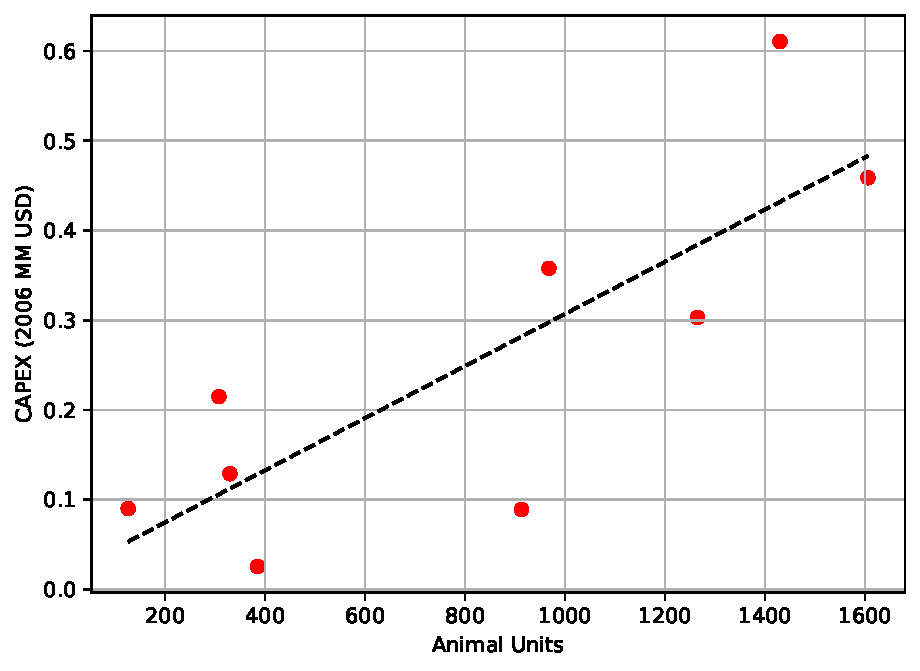
\includegraphics[width=\textwidth, trim={0cm 0cm 0cm 0cm},clip]{gfx/AppendixD/AD_SizeCost_Swine.pdf}
		\caption{Cost of AD units as a function of animal units.}
		\label{fig:AD_SizeCost_Swine}
	\end{subfigure}
	\bigskip
	\begin{subfigure}[t]{0.7\textwidth}
		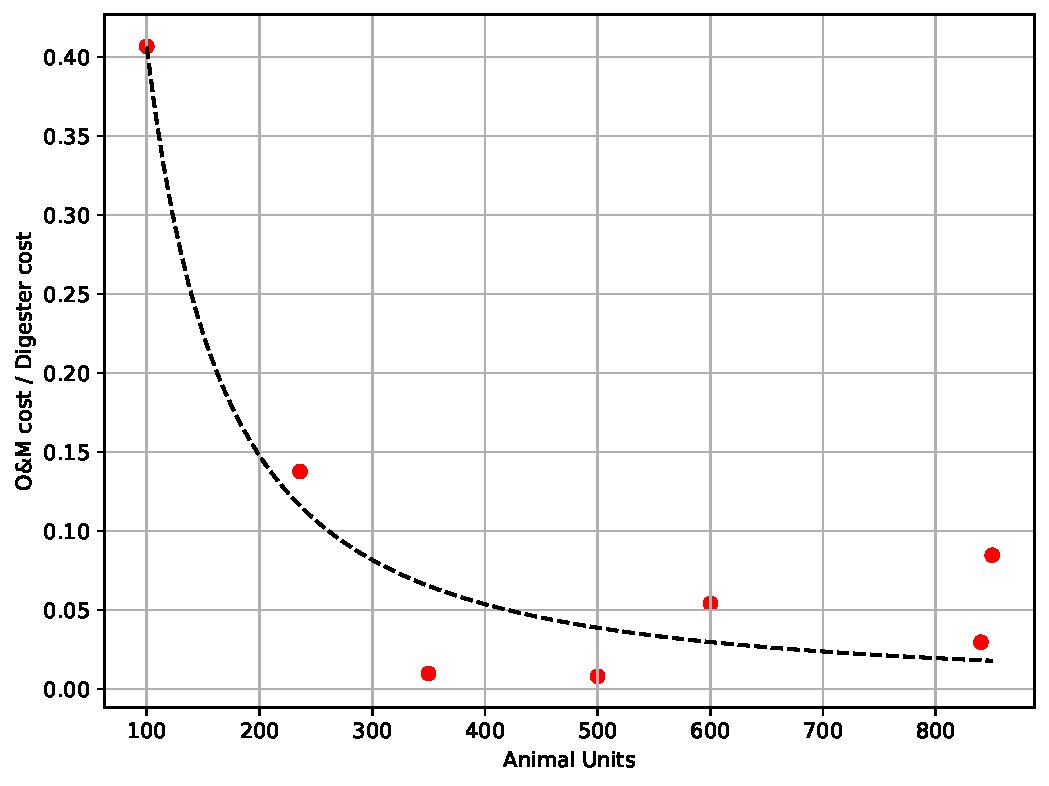
\includegraphics[width=\textwidth]{gfx/AppendixD/AD_size_OM_Unit_cost.pdf} 
		\caption{O\&M costs as a function of animal units.}
		\label{fig:AD_size_OM_Unit_cost}
	\end{subfigure}
	
	\caption{Correlations between AD capital and O\&M costs, and the number of cattle in the livestock facility. Data from \protect\citet{USDA_OM}.}
	\label{fig:AD_size_2cost}
\end{figure}

\subsection{Biogas conditioning}\label{section:BiogasConditioningNRecovery}
\subsubsection{Moisture removal}
The biogas produced contains saturated water at operating temperature. The first stage for water removal is the moisture condensation, which can remove residual dust and oil as well. However, the biogas moisture can remain saturated at the cooled down temperature, and additional disecation stage can be needed, using adsorbent agents such as silica gel or zeolites in packed bed columns operating at pressures between 6 and 10 bar \citep{ryckebosch2011techniqu}.

\subsubsection{H\textsubscript{2}S removal}
Hydrogen sulphide can be removed during the digestion step, or treating the biogas stream leaving the digestor. A review of H\textsubscript{2}S can be found in \citet{ryckebosch2011techniqu}. In this work, in-biogas hydrogen sulphide removal is considered by using a fixed absorbent bed of Fe\textsubscript{2}O\textsubscript{3}, so that hydrogen sulphide is removed in the form of Fe\textsubscript{2}S\textsubscript{3}, as shown in Eq \ref{eq:H2SRemovalNRecovery}. This unit operates at 25-50 ºC. Although is sensitive to the presence of water, it is a high efficient process. Therefore, the moisture removal must be previously performed.

\begin{align}
& \text{Fe\textsubscript{2}O\textsubscript{3}} + 3\text{H\textsubscript{2}S} \rightarrow \text{Fe\textsubscript{2}S\textsubscript{3}} + 3\text{H\textsubscript{2}O} \label{eq:H2SRemovalNRecovery}
\end{align}

The bed can be regenerated using oxygen (air), leading to the formation of elementary sulfur, Eq. \ref{eq:H2SRemovalRegenerationNRecovery}.

\begin{align}
& 2\text{Fe\textsubscript{2}S\textsubscript{3}} + 3\text{O\textsubscript{2}} \rightarrow \text{Fe\textsubscript{2}O\textsubscript{3}} + 6\text{H\textsubscript{2}OS} \label{eq:H2SRemovalRegenerationNRecovery}
\end{align}

\subsubsection{Ammonia removal}
Ammonia contained in biogas can be removed by using adsorption methods such as fixed beds of zeolites or activated carbon, as well as through water scrubbing processes.

\subsection{Digestate solid-liquid separation} \label{section:SLSeparationNRecovery}
Nutrients contained in organic waste (manure or digestate, depending on whether AD is carried out or not) are present in both organic and inorganic forms. Organic nutrients are chemically bound to carbon, and they have to be converted into their inorganic forms through a mineralization process to be available for the vegetation to grow. Organic nutrients are mainly contained in the solid phase of organic waste. Inorganic nutrients are water soluble, and they are mostly present in the liquid phase, or bounded to soluble minerals. They are immediately available to plants, including algae involved in the occurrence of algal blooms. To recover the inorganic fraction of nutrients, a solid-liquid separation stage is implemented, keeping the inorganic nutrients in the liquid stage, which will be further processed, and the organic nutrients in the solid phase, which can be composted to mineralize nitrogen and phosphorus and be further used as fertilizers.

Based on the evaluation reported by \citet{MollerSLsep}, a screw press is the technology selected to carry out the solid-liquid separation stage since it is the most cost efficient solid-liquid separation equipment. The experimental results reported in this study are used to determine the partition coefficients for the different elements, as shown in Table \ref{table:part_coef}.

\begin{table}[h!] 
%	\begin{adjustwidth}{}{}
		\centering
		\caption{Partition coefficients for solid-liquid manure separation using a screw press unit \protect\citep{MollerSLsep}} \label{table:part_coef}
		\resizebox{0.6\columnwidth}{!}{
		\begin{tabular}{c c c}
			\toprule
			Element 	& Solid fraction & Liquid fraction	\\ \midrule
			Total mass 	& 0.08		& 0.92 \\
			Dry matter 	& 0.31		& 0.69 \\
			Org. N 		& 0.09		& 0.91 \\
			Org. P		& 0.22	 	& 0.78 \\ \bottomrule
		\end{tabular}}
%	\end{adjustwidth}
\end{table}

To determine the commercial sizes and number of units necessary as a function of the flow to be treated, data from commercial manufacturers is considered \citep{PWTech}. The feasible configurations in terms of screw press diameter and number of units as a function of the waste flow treated are shown in Table 4 of the Supplementary Material. Data reported by \citet{Matches} for this type of equipment is used to relate the unit diameter and cost, while the operating costs are calculated assuming power consumption reported by the manufacturer for each model, as shown in Fig. \ref{fig:screwpress_investment_costs} and Tables \ref{table:ScrewPress_units} and \ref{table:ScrewPress_power}.

\begin{figure}[h!]
	\centering
	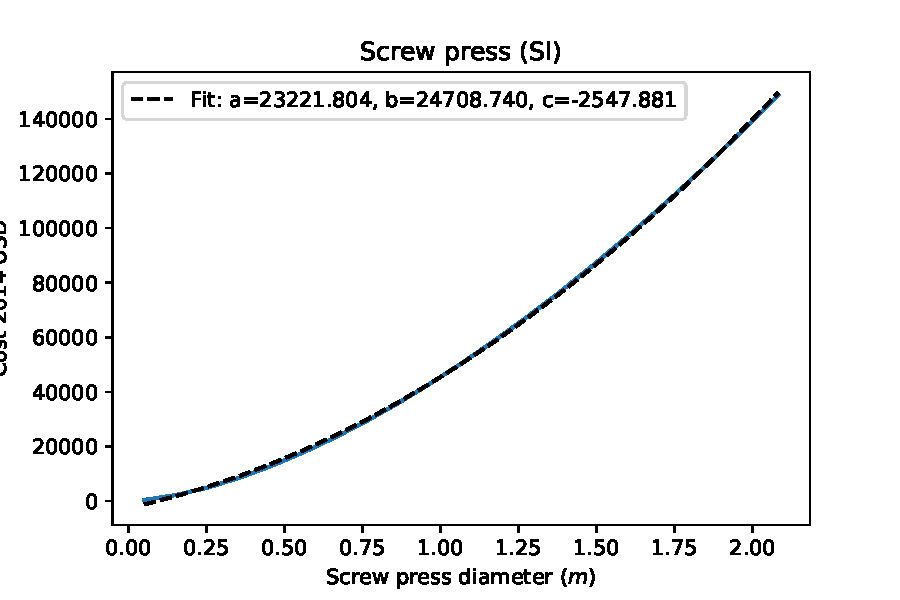
\includegraphics[width=0.8\linewidth, trim={0.5cm 0cm 0cm 0cm},clip]{gfx/AppendixD/screwpress_cost_m} 
	\caption{Estimated screw press investment costs (USD) as a function of the size.}
	\label{fig:screwpress_investment_costs}
\end{figure}

\begin{table}[h!] 
%	\begin{adjustwidth}{}{}
		\centering
		\caption{Sizing estimated for screw press units based on commercial data \protect\citep{PWTech}} \label{table:ScrewPress_units}
		\resizebox{\columnwidth}{!}{
		\begin{tabular}{c c c c c}
			\toprule
			\multicolumn{1}{c}{Load capacity $\left(\frac{m^{3}}{day}\right)$}&\multicolumn{4}{c}{Number of units}\\
			\cmidrule(lr){2-5}
			&\diameter(m) 0.23 & \diameter(m) 0.35 & \diameter(m) 0.42 & \diameter(m) 0.56	\\ \midrule
			$<$ 43 		& 1 	& - 					& - & -	\\
			43 - 81 	& -						& 1 	& - & - 	\\
			81 - 190 	& -						& - 					& 1 & - 	\\
			190 - 381 	& -						& -					 	& 2 & -	\\ 
			381 - 572 & -						& -					 	& 3 & - 	\\ 
			572 - 708 & -						& -					 	& - & 2	 	\\ 
			708 - 1090 & -						& -					 	& - & 3	 	\\
			1090 - 1444 & -						& \-				 	& - & 4	 	\\
			$>$ 1444 	&-						& -					 	& - & $\ceil[\bigg]{\frac{\text{Flow } \left(\sfrac{m^{3}}{day}\right)}{\text{Load Capacity}_{\text{\diameter 0.56m unit}}}}$  	\\\bottomrule
		\end{tabular}}
%	\end{adjustwidth}
\end{table}

\begin{table}[h!] 
%	\begin{adjustwidth}{}{}
		\centering
		\caption{Electrical power of screw press units \protect\citep{PWTech}} \label{table:ScrewPress_power}
		\resizebox{0.85\columnwidth}{!}{
		\begin{tabular}{c c c c c}
			\toprule
			\multicolumn{1}{c}{Number of units } &\multicolumn{4}{c}{Electrical power (kW)}\\
			\cmidrule(lr){2-5}
			&\diameter(m) 0.23 & \diameter(m) 0.35 & \diameter(m) 0.42 & \diameter(m) 0.56	\\ \midrule
			1 		& 0.3 & 0.45 & 0.9 & -	\\
			2 	& -						& - 	& 1.27 & 3.88 	\\
			3	& -						& - 					& 2.01 & 6.34 	\\
			4 	& -						& - 					& - & 7.83 \\
			\bottomrule
		\end{tabular}}
%	\end{adjustwidth}
\end{table}

Assuming the discretization of units due to the commercial sizes available, the investment and operating costs for the screw press equipment are presented in Fig 4 of the Supplementary Material.

\subsection{Struvite production: Multiform system}
Struvite production from livestock waste has been estimated based on a detailed thermodynamic model for precipitates (struvite and calcium compounds) formation considering the main chemical systems involved in the formation of precipitates, shown in Tables \ref{table:pKNitrogenSP} and \ref{table:solids_speciesNitrogenSP}. $pK$ denotes the thermodynamic equilibrium constant, and $pK_{sp}$ refers to the solubility product. The variability in the organic waste composition is also considered, obtaining surrogate models to predict the formation of struvite based on different waste parameters, including the concentration of magnesium, the concentration of calcium, and the alkalinity level \citep{martin2020model}. Based on previous studies, the supply of magnesium has been fixed at a Mg\textsuperscript{2+}/PO\textsuperscript{3-}\textsubscript{4} molar ratio of 2, estimating the formation of struvite as a function of the concentration of Ca\textsuperscript{2+} ions, which compete for phosphate ions hindering the formation of struvite, shown in Eq. \ref{eq:sigmoidal_Ca_StrYield}. A comprehensive description of the thermodynamic model used for the development of the correlations to estimate the formation of struvite can be found in \citet{martin2020model}.

\begin{table}[h!] 
%	\begin{adjustwidth}{}{}
		\centering
		\caption{Aqueous phase chemical systems considered in the thermodynamic model for estimating the formation of struvite.} \label{table:pKNitrogenSP}
		\resizebox{\columnwidth}{!}{
		\begin{tabular}{c c c c}
			\toprule
			Name	& Chemical system &${pK}$	&Source	\\ \midrule
			Ammonia & $\text{NH}_{4}^{+} \leftrightarrow \text{NH}_{3} + \text{H}^{+}$	&9.2 &\citet{Bates}	\\ 
			Water & $\text{H}_{2}\text{O} \leftrightarrow \text{OH}^{-} + \text{H}^{+}$	&14  &\citet{Skoog}	\\ 
			\multirow{3}{*}{Phosphoric acid} & $\text{H}_{3}\text{PO}_{4} \leftrightarrow \text{H}_{2}\text{PO}_{4}^{-} + \text{H}^{+}$	&2.1	&\citet{Ohlinger}	\\ 
			&$\text{H}_{2}\text{PO}_{4}^{-} \leftrightarrow \text{HPO}_{4}^{2-} + \text{H}^{+}$	&7.2  &\citet{Ohlinger}	\\ 
			&$\text{HPO}_{4}^{2-} \leftrightarrow \text{PO}_{4}^{3-} + \text{H}^{+}$	&12.35 &\citet{Ohlinger}	\\ 
			\multirow{2}{*}{Carbonic acid} & $\text{H}_{2}\text{CO}_{3} \leftrightarrow \text{HCO}_{3}^{-} + \text{H}^{+}$	&6.35	&\citet{Skoog}	\\  
			&$\text{HCO}_{3}^{-} \leftrightarrow \text{CO}_{3}^{2-} + \text{H}^{+}$	&10.33	&\citet{Skoog}	\\ \bottomrule
		\end{tabular}}
%	\end{adjustwidth}
\end{table}

\begin{table}[h!] 
%	\begin{adjustwidth}{}{}
		\centering
		\caption{Solids species considered in the thermodynamic model for estimating the formation of struvite.} \label{table:solids_speciesNitrogenSP}
		\resizebox{\columnwidth}{!}{
		\begin{tabular}{c c c c}
			\toprule
			Name	& Chemical system &${pK}_{{sp}}$	&Source	\\ \midrule
			Struvite	& \begin{tabular}[c]{@{}c@{}}$\text{MgNH}_{4}\text{PO}_{4} \cdot 6\text{H}_{2}\text{O} \leftrightarrow$\\ $\text{Mg}^{2+} + \text{NH}_{4}^{+} + \text{PO}_{4}^{3-}$\end{tabular} &13.26 &\citet{Ohlinger} 	\\
			K-struvite	& \begin{tabular}[c]{@{}c@{}}$\text{MgKPO}_{4} \cdot 6\text{H}_{2}\text{O} \leftrightarrow$ \\ $\text{Mg}^{2+} + \text{K}^{+} + \text{PO}_{4}^{3-}$\end{tabular} & 10.6 & \citet{TaylorAW}  	\\ 
			Hydroxyapatite	& \begin{tabular}[c]{@{}c@{}}$\text{Ca}_{5} \left( \text{PO}_{4} \right)_{3}\text{OH} \leftrightarrow$\\ $5\text{Ca}^{2+} + 3\text{PO}_{4}^{3-}+\text{OH}^{-}$\end{tabular} &44.33 &\citet{Brezonik}  \\ 
			Calcium carbonate	& $\text{CaCO}_{3} \leftrightarrow \text{Ca}^{2+} + \text{CO}_{3}^{2-}$ &8.48	&\citet{Morse} \\ 
			Tricalcium phosphate	& $\text{Ca}_{3} \left( \text{PO}_{4} \right)_{2} \leftrightarrow 3\text{Ca}^{2+} + 2\text{PO}_{4}^{3-}$ &25.50 &\citet{Fowler} 	\\
			Dicalcium phosphate	& $\text{CaHPO}_{4} \leftrightarrow \text{Ca}^{2+} + \text{HPO}_{4}^{2-}$ &6.57	&\citet{Gregory} 	\\
			Calcium hydroxide	& $\text{Ca} \left( \text{OH} \right)_{2} \leftrightarrow \text{Ca}^{2+} + 2\text{OH}^{-}$ &5.19  &\citet{Skoog}  \\
			Magnesium hydroxide	& $\text{Mg(OH)}_{2} \leftrightarrow \text{Mg}^{2+} + 2\text{OH}^{-}$&11.15  &\citet{Skoog} 	\\  \bottomrule 
		\end{tabular}
%	\end{adjustwidth}
}
\end{table}

A correlation
%developed in a previous work has been used to compute
to estimate the formation of struvite through the fraction of phosphorus recovered as struvite $\left(x_{\text{struvite} \left(\text{PO}_{4}^{3-}\right) }\right) $ as a function of calcium concentration in the waste has been used in this work, Eq. \ref{eq:sigmoidal_Ca_StrYield} \citep{martin2020model}.
% \ref{table:pK}, as well as the thermodynamic equilibrium constant of each equilibrium ($p_K$).
Based on the correlation shown in Eq. \ref{eq:sigmoidal_Ca_StrYield}, the amount of nitrogen recovered is estimated through Eq. \ref{eq:N_Multiform}.

\begin{align}
& x_{\text{struvite} \left(\text{PO}_{4}^{3-}\right) }= \frac{0.798}{1+\left(x_{\text{Ca}^{2+}:\text{PO}_{4}^{3-}} \cdot 0.576\right)^{2.113}} \label{eq:sigmoidal_Ca_StrYield}
\\
& \dot{m}_{\text{struvite } recovered} = \dot{m}_{\text{P } in}  \cdot x_{\text{struvite} \left(\text{PO}_{4}^{3-}\right) } \cdot \frac{MW_{\text{struvite}}}{MW_{\text{P}}}
\\
& \dot{m}_{\text{N } recovered} =  \dot{m}_{\text{struvite } recovered} \cdot \frac{MW_{\text{N}}}{MW_{\text{struvite}}} \label{eq:N_Multiform}
\\ 
& \dot{m}_{\text{N } released} = \dot{m}_{\text{N } in} - \dot{m}_{\text{struvite } recovered} \cdot \frac{MW_{\text{N}}}{MW_{\text{struvite}}}
\end{align} 

\subsection{MAPHEX}
The mass balances of MAPHEX process are shown in Eqs. \ref{eq:MAPHEX1}-\ref{eq:MAPHEX5}, based on experimental data for full-scale modular units reported by \citet{church_versatility2018}.

\begin{align}
& \dot{m}_{nutrients_\text{recovered}} = \dot{m}_{nutrients, \ in} \cdot \eta_{\text{MAPHEX}}^{{nutrients}}, \label{eq:MAPHEX1} \\
& \forall \ nutrients \ \in \ \{\text{P}, \ \text{N}\} \nonumber
\\
& \dot{m}_{nutrients_\text{released}} = \dot{m}_{nutrients, \ in} \cdot \left(1- \eta_{\text{MAPHEX}}^{{nutrients}}\right), \label{eq:MAPHEX2} \\
& \forall \ nutrients \ \in \ \{\text{P}, \ \text{N}\}  \nonumber
%	\nonumber
\\
& \dot{m}_{\text{TS\textsubscript{recovered}}} = \dot{m}_{\text{TS}, in} \cdot 0.93 \label{eq:MAPHEX3}
\\
& \dot{m}_{\text{water\textsubscript{recovered}}} = \frac{\dot{m}_{\text{TS\textsubscript{recovered}}}}{0.25} \cdot 0.75 \label{eq:MAPHEX4}
\\
& \dot{m}_{\text{water\textsubscript{released}}} = \dot{m}_{\text{water}, in} - \dot{m}_{\text{water\textsubscript{recovered}}} \label{eq:MAPHEX5}
\end{align}

\subsection{Transmembrane chemisorption}
Characteristics of Liquid-Cel\textsuperscript{\texttrademark} Extra Flow membranes are shown in Table \ref{table:membrane_characteristichs}. Membrane modules cost are illustrated in Figure \ref{fig:MembranesCostNitrogenSM}.

\begin{table}[h] 
	\centering
	\caption{Main characteristics of Liquid-Cel \textsuperscript{\texttrademark} membrane \protect\citep{rongwong2020modelin, ulbricht2013ammoni}.} \label{table:membrane_characteristichs}
	%	\begin{threeparttable}
	\resizebox{0.8\columnwidth}{!}{
	\begin{tabular}{@{}cccc@{}}
		\toprule
		Membrane parameters  & Unit & Variable & Values  \\ \midrule
		Number of fibers     & $\frac{\text{fibers}}{\text{m}^2_{\text{module}}}$    & $n_f$       & $2.13 \cdot 10^6$    \\
		Fiber outer diameter & m    & $d_o$       & $300 \cdot 10^{-6}$  \\
		Fiber inner diameter & m    & $d_i$       & $240 \cdot 10^{-6}$  \\
		Pore diameter        & m    & $a$         & $0.04 \cdot 10^{-6}$ \\
		Porosity             & -    & $\varepsilon$  & 0.40     \\
		Tortuosity factor    & -    & $\tau$      & 2.60     \\
		Pressure drop shell side    & bar    & $\Delta P_{\text{shell side}}$      & 0.3     \\
		Pressure drop lumen side    & bar    & $\Delta P_{\text{lumen side}}$      & 2     \\
		\bottomrule
	\end{tabular}}
\end{table}

\begin{figure}[h!]
	\centering
	%	\begin{subfigure}[t]{0.5\linewidth}
	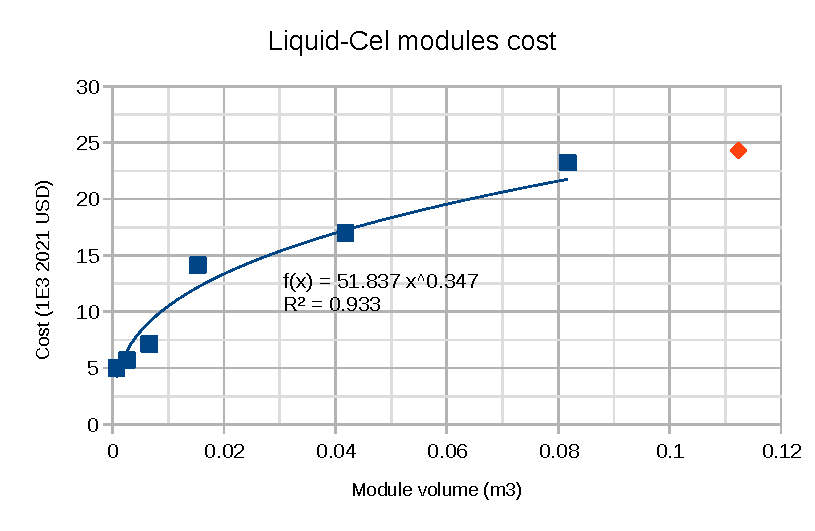
\includegraphics[width=0.8\linewidth, trim={0cm 0cm 0cm 0cm},clip]{gfx/AppendixD/MembranesCost.pdf} 
	\caption{Estimation of Liquid-Cel\textsuperscript{\texttrademark} 14x40 membrane module cost.}
	\label{fig:MembranesCostNitrogenSM}
\end{figure}

The main parameters for membrane modeling are collected in Eqs. \ref{eq:Mem1}-\ref{eq:Mem99}. Digestate density ($\rho$) and ($\mu$) viscosity were assumed equal to those of water. Correlations to estimate these parameters are reported by \citet{hsu1997densities}. Ammonia Henry's constant ($H_{\text{NH}_3}$)
%and  Knudsen diffusivity 
have been taken from \citet{linstrom2001nist}.

\begin{align}
& \rho_{\text{water}} \left(\frac{\text{kg}}{\text{m}^3}\right) = (10^3) \cdot \nonumber \\
& \left(0.863559+1.21494 \cdot 10^{-3} \cdot T(\text{K}) - 2.5708 \cdot 10^{-6} \cdot T(\text{K})^2\right) \label{eq:Mem1} 
\\
& \mu_{\text{water}} \left(\frac{\text{kg}}{\text{m} \cdot \text{s}}\right) = (10^{-6}) \cdot \left(\rho \cdot e^{-3.28285+\frac{456.029}{T(\text{K})-154.576}}\right) \label{eq:Mem2} 
\\
& H_{\text{NH}_3} \left(\frac{\text{kmol}}{\text{atm} \cdot \text{m}^3}\right) = 58 \cdot e^{4100 \cdot \left(\frac{1}{T(\text{K})} - \frac{1}{298.15}\right)}
\label{eq:Mem3}
\end{align}

The cross-sectional area of the lumen area is calculated based on the transverse area of hollow fiber, and the number of fibers in the membrane module, Eq. \ref{eq:A_lumen} . Shell area is calculated as the difference between total and lumen side cross-sectional areas. 
Velocities of digestate and stripping fluid (i.e., sulfuric acid solution) are computed based on their respective volumetric flow and transverse areas.

\begin{align}
& n_{f_{\text{module}}} = A_{\text{module}} \cdot n_f \label{eq:Memnf} 
\\
& A_{\text{lumen side}} \left(\text{m}^2\right) = \frac{d_i^2}{4} \cdot \pi \cdot n_{f_{\text{module}}} \label{eq:A_lumen} 
\\
& A_{\text{shell side}} \left(\text{m}^2\right) = \frac{D_{\text{module}^2}}{4} \cdot \pi - A_{\text{lumen side}} \label{eq:A_shell} 
\\
& V_{\text{stripping fluid}} \left(\frac{\text{m}}{\text{s}}\right) = \frac{\dot{V}_{\text{stripping fluid}}}{A_{\text{lumen side}}} \label{eq:V_stripping}
\\
& V_{\text{digestate}} \left(\frac{\text{m}}{\text{s}}\right) = \frac{\dot{V}_{\text{digestate}}}{A_{\text{shell side}}} \label{eq:V_digestate}
\end{align}

Diffusion of ammonia through the membrane is driven by bulk and Knudsen diffusivities, which consider the mean free path of molecules and the pore diameter respectively. Bulk diffusivity of ammonia is calculated based on the kinetic theory, using Eq. \ref{eq:Mem5}, while Knudsen diffusivity depends on the molecular velocity, Eq. \ref{eq:Mem4}, and pore diameter, Eq. \ref{eq:Mem7} \citet{agrahari2012model}. Both contributions to ammonia transport are combined in an effective diffusion coefficient, Eq. \ref{eq:Mem88}. Ammonia diffusion in liquid phase has been assumed equal to ammonia diffusion in water, which is calculated using Eq. \ref{eq:Mem99}. 

\begin{align}
& \bar{v}  \left(\frac{\text{m}}{\text{s}}\right) = \left(\frac{8 \cdot R\left(\frac{\text{J}}{\text{mol} \cdot \text{K}}\right) \cdot T\left(\text{K}\right)}{MW_{\text{NH}_3} \left(\frac{\text{kg}}{\text{mol}}\right) \cdot \pi} \right)^{\sfrac{1}{2}}
\label{eq:Mem4} 
\\
& D_{\text{NH}_{3}}  \left(\frac{\text{m}^2}{\text{s}}\right) = \frac{1}{3} \cdot \lambda \cdot \bar{v}
\label{eq:Mem5} 
\\
& \lambda  \left(\text{m}\right) = \frac{\kappa \left(\frac{\text{J}}{\text{K}}\right) \cdot T\left(\text{K}\right)}{\pi \cdot \sigma_{\text{NH}_3}^2 \left(\text{m}^2\right) \cdot P\left(\text{Pa}\right) \cdot 2^{\sfrac{1}{2}}}
\label{eq:Mem6} 
\\
& D_{\text{NH}_{3_\text{Kn}}} \left(\frac{\text{m}^2}{\text{s}}\right) = \frac{d_{\text{pore}}}{3} \cdot \left(\frac{8 \cdot R\left(\frac{\text{J}}{\text{mol} \cdot \text{K}}\right) \cdot T(\text{K})} {\pi \cdot MW_{\text{NH}_3} \left(\frac{\text{kg}}{\text{mol}}\right)} \right)^{\sfrac{1}{2}}
\label{eq:Mem7}
\\
& D_{\text{eff}} \left(\frac{\text{m}^2}{\text{s}}\right) = \frac{1}{\frac{1}{D_{\text{NH}_{3_\text{Kn}}}} + \frac{1}{D_{\text{NH}_{3}}}}
\label{eq:Mem88}
\\
& D_{\text{NH}_{3_\text{water}}} \left(\frac{\text{m}^2}{\text{s}}\right) = 1.96 \cdot 10^{-9} \cdot \frac{\mu_{\text{water}_{T=298\text{K}}}}{\mu_{\text{water}_{T}}} \cdot \frac{T\left(\text{K}\right)}{298}
\label{eq:Mem99}
\end{align}

The distribution of ammonia species shown in Eq. \ref{eq:NH3NH4} is calculated at initial conditions based on the pH of the digestate stream being fed through the tube side of the membrane module, which is assumed equal to 11, as shown in Eqs. \ref{eq:Mem8}-\ref{eq:Mem12}.

\begin{align}
&  f_{\text{NH}_3} = \frac{1}{10^{\left(pK_{a_{\text{NH}_3}}-pH\right)}+1} \label{eq:Mem8} 
\\
&  pK_{a_{\text{NH}_3}} \left(\frac{\text{kmol}}{\text{m}^3}\right) = 0.0901821+\frac{2729.92}{T(\text{K})} \label{eq:Mem11} 
\\
&  \left[{\text{NH}_3}\right] = \left[{\text{N}_\text{inorg}}\right] \cdot f_{\text{NH}_3} \label{eq:Mem9} 
\\
&  \left[{\text{NH}_4^+}\right] = \left[{\text{N}_\text{inorg}}\right] \cdot \left(1-f_{\text{NH}_3}\right) \label{eq:Mem10} 
\\
&  \left[{\text{H}^+}\right] = K_a \cdot \frac{\left[{\text{NH}_4^+}\right]}{\left[{\text{NH}_3}\right]} \label{eq:Mem12} 
\end{align}

A modified Henry's constant considering the speciation of ammonia is used in the model proposed by \citet{rongwong2020modelin} to evaluate the liquid-solid equilibrium of ammonia, Eq. \ref{eq:Mem13}.

\begin{align}
&  H_{\text{NH}_3}^* = H_{\text{NH}_3} \cdot \left(1+\frac{K_a \cdot \left[{\text{H}^+}\right]}{Kw}\right) \label{eq:Mem13}  
\end{align}

The mass transfer coefficient of the digestate flowing in the tube side, $k_{\text{digestate}}$, is calculated through the Sherwood number of this stream, Eq. \ref{eq:Mem14}.
\begin{align}
&  \text{Sh}_{\text{digestate}} = \frac{k_{\text{digestate}} \cdot d_i}{D_{\text{NH}_{3_\text{water}}}} = \label{eq:Mem14} \\
& 1.62 \cdot \left(\frac{d_i}{L} \cdot \text{Re}_{\text{digestate}} \cdot \text{Sc}_{\text{digestate}}\right)^{\sfrac{1}{3}} \nonumber
\\
&  \text{Re}_{\text{digestate}} = \frac{d_i \cdot \rho_{\text{digestate}} \cdot V_{\text{digestate}}}{\mu_{\text{digestate}}} \label{eq:Mem15}
\\
&  \text{Sc}_{\text{digestate}} = \frac{\mu_{\text{digestate}}}{\rho_{\text{digestate}} \cdot D_{\text{NH}_{3_\text{water}}}} \label{eq:Mem16}
\end{align}

The membrane phase can be divided into non-wetted and wetted membrane sections. Their mass transfers coefficients, $k_M$ and $k_M^{'}$ respectively, are calculated based on the fraction of membrane wetted by the digestate. This is calculated based on a correlation reported by \citet{rongwong2020modelin}, shown in Eq. \ref{eq:Mem20}. Eqs. \ref{eq:Mem17}-\ref{eq:Mem18} and \ref{eq:Mem21}-\ref{eq:Mem22} shown the equations employed for the estimation of $k_M$ and $k_M^{'}$ respectively.
\begin{align}
& w_{\text{membrane}} = \frac{0.368}{2.709 + e^{-17.486 \cdot \left(V_{\text{digestate}}-0.25\right)}} \label{eq:Mem20}
\\
& d_{\text{interfacial}} \left(\text{m}\right) = d_i + w_{\text{membrane}} \cdot \left(d_o-d_i\right) \label{eq:Mem19}
\\
&  k_M \left(\frac{\text{m}}{\text{s}}\right) = \frac{D_{\text{eff}} \cdot \varepsilon}{\tau \cdot \delta_{\text{non-wetted}}} \label{eq:Mem17}
\\
& \delta_{\text{non-wetted}} \left(\text{m}\right) = \frac{d_o-d_{\text{interfacial}}}{2} \label{eq:Mem18}
\\
&  k_M^{'} \left(\frac{\text{m}}{\text{s}}\right) = \frac{D_{\text{water}} \cdot \varepsilon}{\tau \cdot \delta_{\text{wetted}}} \label{eq:Mem21}
\\
& \delta_{\text{wetted}} \left(\text{m}\right) = \frac{d_{\text{interfacial}}-d_i}{2} \label{eq:Mem22}
\end{align}

The overall mass transfer coefficient is calculated based on the liquid, wetted membrane, and non-wetted membranes mass transfer coefficients, as shown in Eq. \ref{eq:Mem23}. However, high ammonia concentrations result in a decrease of the overall mass transfer \citep{zhu2005modified}. Therefore, $K_{ov}$ is modified using a correction factor that consider the concentration of ammonia in digestate.

\begin{align}
& K_{ov} \left(\frac{\text{m}}{\text{s}}\right) = \frac{1}{\left(\frac{1}{k_{\text{digestate}} \cdot d_i} + \frac{1}{k_M^{'} \cdot \delta_{\text{ln wetted}}} + \frac{R \left(\frac{\text{atm} \cdot \text{m}^3}{\text{kmol} \cdot \text{K}}\right) \cdot T(\text{K}) \cdot H_{\text{NH}_3}^{*}}{k_M \delta_{\text{ln non-wetted}}}\right) \cdot d_o } \label{eq:Mem23}
\\
& \delta_{\text{ln wetted}} = \frac{d_{\text{interfacial}}-d_i}{\text{ln}\left( \frac{d_{\text{interfacial}}}{d_i}\right)} \label{eq:Mem24}
\\
& \delta_{\text{ln non-wetted}} = \frac{d_o - d_{\text{interfacial}}}{\text{ln}\left( \frac{d_o}{d_{\text{interfacial}}}\right)} \label{eq:Mem25}
\\
& K_{ov_{\text{corrected}}} \left(\frac{\text{m}}{\text{s}}\right) = K_{ov} \cdot \left(1-\frac{0.002728 \cdot \left[\text{NH}_3\right] \left(\frac{\text{mg}}{\text{L}}\right)}{100}\right) \label{eq:KovCorrected}
\end{align}

The mass balance along the membrane can be performed considering the mass transfer in an infinitesimal element of the membrane, as shown in Eq. \ref{eq:Mem26}. Due to the excess of sulfuric acid in the lumen side that lead to the formation of ammonium sulfate from the ammonia recovered, the concentration of ammonia in the lumen side is assumed negligible. This differential expression can be analytically integrated to estimate the total length of the membrane, Eq. \ref{eq:Mem27}.

\begin{align}
\frac{\dot{n}_{\text{NH}_3}}{dz} &= -n_{f_{\text{module}}} \cdot \pi \cdot d_o \cdot K_{{ov}_\text{corrected}} \cdot \left( \frac{\dot{n}_{\text{NH}_3}}{\dot{V}_{\text{digestate}}} - \frac{ H_{\text{NH}_3}^* \cdot p_{\text{NH}_3}}{\dot{V}_{\text{digestate}}}\right) \nonumber
\\ 
& \approx -n_{f_{\text{module}}} \cdot \pi \cdot d_o \cdot K_{{ov}_\text{corrected}} \cdot \frac{\dot{n}_{\text{NH}_3}}{\dot{V}_{\text{digestate}}} \label{eq:Mem26}
\\
& z \left(\text{m}\right) = \text{ln}\left(\frac{\dot{n}_{\text{NH}_{3_{final}}}}{\dot{n}_{\text{NH}_{3_{initial}}}}\right) \cdot \frac{\dot{V}_{\text{digestate}}}{-n_{f_{\text{module}}} \cdot \pi \cdot d_o \cdot K_{{ov}_\text{corrected}}} \label{eq:Mem27}
\end{align}

%Additionally, 
Pumps to drive the digestate and stripping fluid streams are needed. Their cost is estimated using Eqs. \ref{eq:n_pumps} and \ref{eq:pumpsCAPEX}, assuming that the maximum capacity of one single pump $\left(\dot{V}_{\text{pump}_{\text{max}}}\right)$ is 1 $\sfrac{\text{m}^3}{\text{s}}$ \citep{peters2003plant}. Pumps operating cost are estimated through Eqs. \ref{eq:pumpsH} to \ref{eq:pumpsOPEX}, calculating the energy needed to balance the pressure drop of the shell and lumen sides of the membrane, Table \ref{table:membrane_characteristichs}. Pump efficiencies $\left(\eta_{\text{pump}_i}\right)$ of 0.8 are assumed.
\begin{align}	
&
n_{\text{pump}_i} = \ceil*{\frac{\dot{V}_i}{\dot{V}_{\text{pump}_{\text{max}}}}} \label{eq:n_pumps}
\\
& CAPEX_{\text{pumps}_i} \left(\text{2019 USD}\right) = \nonumber \\
&
\begin{cases}
(-50.387\cdot10^6 \cdot \dot{V}_i^2 + 1.607\cdot10^6 \cdot \dot{V}_i 
\\
+ 5.127\cdot10^3) \cdot n_{\text{pump}_i} \cdot 1.055 & \text{if } \dot{V}_i \leq 9\cdot10^{-3} \frac{\text{m}^3}{\text{s}}  \\
(92.562\cdot10^3\cdot \dot{V}_i^{0.381}) \cdot n_{\text{pump}_i} \cdot 1.055 & \text{if }  \dot{V}_i > 9\cdot10^{-3} \frac{\text{m}^3}{\text{h}}
\end{cases} \label{eq:pumpsCAPEX} \\ 
& H_i \left(\text{m}\right) = \frac{\Delta P_i \left(\text{Pa}\right)}{\rho \left(\frac{\text{kg}}{\text{m}^3}\right) g\left(\frac{\text{m}}{\text{s}^2}\right)} \label{eq:pumpsH}
\\
& \dot{W}_{\text{pump}_i} \left(\text{kW}\right) = \frac{g\left(\frac{\text{m}}{\text{s}^2}\right) \cdot H_i \left(\text{m}\right) \cdot \rho \left(\frac{\text{kg}}{\text{m}^3}\right) \cdot \dot{V}_i \left(\frac{\text{m}^3}{\text{s}}\right)}{\eta_{\text{pump}_i}} \label{eq:pumpsPower}
\\
& OPEX_{\text{pumps}} \left(\frac{\text{2019 USD}}{\text{year}}\right) = \sum_{i} \dot{W}_{\text{pump}_i} \left(\text{kW}\right) \cdot t_{\text{operation}} \left(\text{s}\right) \cdot 3600 \nonumber \\
& \cdot Price_{\text{electricity}}\left(\frac{\text{USD}}{\text{kWh}}\right) \forall \ i  \in \{\text{shellside, lumenside}\} \label{eq:pumpsOPEX} 
\end{align}

\subsection{Ammonia evaporation}\label{section:DigDryingNRecoveryPaper}
The following assumptions have been made for the modeling of digestate drying:
\begin{itemize}
	\item $c_{p_{\text{digestate}_{\text{in}}}} \approx c_{p_{\text{water}}}$
	\item $P_{\text{water}} + P_{\text{NH}_3} \approx P_{\text{water}}$
	\item $T_{\text{out}_{\text{air}}} = T_{\text{out}_{\text{digestate}}}$
	\item $\alpha = \text{constant}$
\end{itemize}

The mass and energy balances for digestate drying in a belt dryer unit are shown in Eqs. \ref{eq:BD11}-\ref{eq:BD15} and \ref{eq:BD1}-\ref{eq:BD10} respectively

\begin{align}
%	& \alpha \cdot \text{ln}\frac{\dot{n}_{\text{water}_\text{in}}}{\dot{n}_{\text{water}_\text{out}}} =  \text{ln}\frac{\dot{n}_{\text{NH\textsubscript{3}}_\text{in}}}{\dot{n}_{\text{NH\textsubscript{3}}_\text{out}}} \label{eq:BD11} 
%	\\
%	& \alpha =  \frac{Pv_{\text{NH}_3} \left(T\right)}{Pv_{\text{water}} \left(T\right)} \label{eq:BD12} 
%	\\
&\dot{m}_{\text{NH}_{3\text{ evap}}} = \dot{m}_{\text{NH}_{3\text{ in}}} \cdot \eta_{\text{belt dryer}}^{\text{NH}_3} \label{eq:BD11} 
\\
& \frac{\frac{\dot{m}_{\text{water}_\text{evap}}}{MW_{\text{water}}}}{\sum_{j}\frac{\dot{m}_j}{MW_j}} \cdot P_{\text{total}} \leq Pv_{\text{water}} \left(T\right) \ \forall \ j \ \in \ \{\text{air}, \ \text{H\textsubscript{2}O}, \ \text{NH}_3\} \label{eq:BD13} 
\\
%	& P_{\text{water}} =  \dot{n}_{\text{water}_\text{evap}} \cdot P_{\text{total}} \label{eq:BD14} 
%	\\
&\frac{\frac{\dot{m}_{\text{NH}_{3\text{ evap}}}}{MW_{\text{NH}_3}}}{\sum_{j}\frac{\dot{m}_j}{MW_j}} \leq Pv_{\text{NH}_3} \left(T\right) \ \forall \ j \ \in \ \{\text{air}, \ \text{H\textsubscript{2}O}, \ \text{NH}_3\}\label{eq:BD15} 
%	\\
%	& \forall \ j \ \in \ \{\text{air}, \ \text{H\textsubscript{2}O}, \ \text{NH}_3\} \nonumber
\end{align}

\begin{align}
& \dot{Q}_{\text{Belt Dryer}} = \dot{H}_{\text{latent}} + \dot{H}_{\text{sensible}} = \dot{H}_{\text{air}_{\text{in}}} - \dot{H}_{\text{air}_{\text{out}}} \label{eq:BD1} 
\\
& \dot{H}_{\text{latent}} = \dot{m}_{\text{water}_\text{evap}} \cdot \lambda_{\text{evap}_{\text{water}}}\left(T\right) + \dot{m}_{\text{NH}_{3_\text{evap}}} \cdot \lambda_{\text{evap}_{\text{NH}_3}}\left(T\right) \label{eq:BD2} 
\\
& \dot{H}_{\text{sensible}} = \dot{H}_{\text{digestate}_\text{out}} - \dot{H}_{\text{digestate}_\text{in}} + \dot{H}_{\text{sensible}_{\text{gases}}} \label{eq:BD3} \\
& \dot{H}_{\text{sensible}_{\text{gases}}} = \left( \dot{m}_{\text{water}_\text{evap}} + \dot{m}_{\text{NH}_{3_\text{evap}}} \right) \cdot c_{p_{\text{water (liquid)}}} \cdot T_{\text{air}_\text{out}} \label{eq:BD4} 
\\
& \dot{H}_{\text{digestate}_{\text{in}}} = \dot{m}_{\text{digestate}_{\text{in}}} \cdot c_{p_{\text{water}}} \cdot \Delta T_{\text{digestate}_\text{in}} \label{eq:BD5} 
\\
& \dot{H}_{\text{digestate}_{\text{out}}} = \dot{m}_{\text{digestate}_{\text{out}}} \cdot c_{p_{\text{digestate}}} \cdot \Delta T_{\text{digestate}_\text{out}} \label{eq:BD6} 
\\
& c_{p_{\text{digestate}}} \left(\sfrac{kg}{kJ \cdot K}\right)= 4.19-0.0275 \cdot \left(\frac{\dot{m}_{\text{TS}_{\text{out}}}}{\dot{m}_{\text{digestate}_{\text{out}}}} \cdot 100 \right) \label{eq:BD7} 
\\	
& \dot{H}_{\text{air}_{\text{in}}} = \dot{m}_{\text{air}} \cdot c_{p_{\text{air}}} \cdot \Delta T_{\text{air}_\text{in}} \label{eq:BD8} 
\\	
& \dot{H}_{\text{air}_{\text{out}}} = \label{eq:BD9} \\
& \left(\dot{m}_{\text{air}} \cdot c_{p_{\text{air}}} + \dot{m}_{\text{water}_\text{evap}} \cdot c_{p_{\text{water (gas)}}} + \dot{m}_{\text{NH}_{3_\text{evap}}} \cdot c_{p_{\text{NH\textsubscript{3} (gas)}}} \right) \cdot \Delta T_{\text{air}_\text{out}} \nonumber 
\\	
& \Delta T_i = T_i - T_\text{ref} \ \forall \ i \ \in \ \{\text{air}_\text{in}, \ \text{air}_\text{out},  \ \text{digestate}_\text{in}, \ \text{digestate}_\text{out} \} \label{eq:BD10}
\end{align}

\subsection{Stripping in packed tower}
The
%theoretical
liquid mass velocity is a known parameter since it corresponds to the digestate being processed. The
%theoretical
gas velocity is estimated by combining Eqs. \ref{eq:PDrop}, \ref{eq:FloodingALAMO} and \ref{eq:OpLine}. The design gas mass velocity considered is 0.7 time the
%theoretical
gas mass velocity, Eq \ref{eq:G_Design}, while the liquid design mass velocity is computed by combining Eqs. \ref{eq:G_Design} and \ref{eq:OpLine}. Tower diameter is computed based on the design liquid mass velocity and liquid mass flow. However, design restrictions reported by \citep{Branan2005} have been considered in the sizing of the packed tower.
Tower height is estimated through the height and number of transfer units, Eqs \ref{eq:DRestriction} and \ref{eq:ZRestriction}. Therefore, the design diameter is computed as shown in Eqs. \ref{eq:A_Stripping} to \ref{eq:StrippingDdesign}. Additionally, the number of packed towers that have to be installed in-parallel arrangement is estimated through Eq. \ref{eq:nStrippers}.

\begin{align}
&D_{\text{design}} \leq 1.2 \text{ m}  \label{eq:DRestriction}\\
& \frac{H_{\text{design}}}{D_{\text{design}}} \leq 30 \label{eq:ZRestriction}\\
& A_{\text{stripping tower}} = \frac{\dot{m}_L}{G_{L_{\text{design}}}} \label{eq:A_Stripping} \\
& D_{\text{stripping tower}} = \left(\frac{A_{\text{stripping tower}}}{\pi}\right)^{0.5} \label{eq:D_Stripping} \\
& D_{\text{stripping tower}}^{\text{design}} \left(\text{m}\right) =
\begin{cases}
D_{\text{stripping tower}} & \text{if } 	D_{\text{stripping tower}} \leq 1.2 \text{ m}  
\\
1.2 & \text{if }  D_{\text{scrubber}} > 1.2 \text{ m}
\end{cases} \label{eq:StrippingDdesign} \\
& n_{\text{stripping tower}}^{\text{parallel}} = \ceil*{\frac{D_{\text{stripping tower}}(\text{m})}{1.2}}\label{eq:nStrippers}
\end{align}

The height of the stripping packed towers is estimated through the height and number of transfer units, Eq. \ref{eq:HTUStripping} and \ref{eq:NTUStripping} respectively \citep{Metcalf2014}. The liquid overall mass transfer coefficient value assumed for the ammonia air system is 2 h\textsuperscript{-1} \citep{larsen2013so}. The design restriction shown in Eq. \ref{eq:ZRestriction} is considered to compute the design height of the stripping towers, and the number of units that must be installed in series, Eq. \ref{eq:nStrippersSerie}.

\allowdisplaybreaks
\begin{align}
& HTU = \frac{\frac{\dot{m}_L}{n_{\text{stripping tower}}^{\text{parallel}} \cdot\rho_{\text{digestate}}}}{K_{L}a \cdot \pi \cdot \left(\frac{D_{\text{stripping tower}}}{2}\right)^2} \label{eq:HTUStripping} \\
& NTU = \frac{S}{S-1} \text{ln}\left(\frac{\frac{1}{1-\sfrac{\eta_{\text{stripping tower}}}{100}} \cdot \left(S-1\right) + 1}{S}\right) \label{eq:NTUStripping} \\
& S = \frac{H_{\text{NH}_3}}{P_{\text{stripping tower}}} \cdot \frac{\dot{m}_G}{\dot{m}_L} \\
& H_{\text{stripping tower}} = NTU \cdot HTU \label{eq:HStripping} \\
& n_{\text{stripping tower}}^{\text{series}} = \ceil*{\frac{\frac{H_{\text{stripping tower}}}{ D_{\text{stripping tower}}^{\text{design}}}}{30}}\label{eq:nStrippersSerie}\\
& H_{\text{stripping tower}}^{\text{design}} \left(\text{m}\right) =
\begin{cases}
H_{\text{stripping tower}} & \text{if } 	\frac{H_{\text{stripping tower}}}{D_{\text{stripping tower}}} \leq 30  
\\
\frac{\frac{\dot{m}_L}{n_{\text{stripping tower}}^{\text{series}} \cdot n_{\text{stripping tower}}^{\text{parallel}} \cdot\rho_{\text{digestate}}}}{K_{L}a \cdot \pi \cdot \left(\frac{D_{\text{stripping tower}}}{2}\right)^2} & \text{if } 	\frac{H_{\text{stripping tower}}}{D_{\text{stripping tower}}} \leq 30  
\end{cases} \label{eq:Stripping2Ddesign}
\end{align}

\subsection{Acidic scrubbing}\label{section:AcidicScrubbingNRecoveryPaper}
Mass balances to scrubber unit consider the water transferred to the gas stream, assuming that saturation is reached, Eq. \ref{eq:SC2}. Ammonia  recovery efficiency ($\eta_{scrubber}^{\text{NH}_3}$) of full-scale ammonia scrubbers has been reported in the range of 40\% to 99\% \citep{melse2005air}. A typical $\eta_{scrubber}^{\text{NH}_3}$ of 96\% has been selected based on the work of \citet{melse2005air}.

\begin{align}
& \frac{P_{\text{water}}}{Pv_{\text{water}}} = 1 \label{eq:SC1} 
\\
& Pv_{\text{water}} = \frac{\frac{\dot{m}_{\text{water}_{out}}^{\text{gas stream}}}{MW_\text{water}}}
{\sum_{j}\frac{\dot{m}_{\text{j}}^{\text{gas stream}}}{MW_\text{j}}}
\cdot P_{in}^{\text{gas stream}} \label{eq:SC2} 
\\
& \dot{m}_{\text{NH}_{3 \ out}}^{\text{gas stream}} = \dot{m}_{\text{NH}_{3 \ in}}^{\text{gas stream}} \cdot \left(1-\eta_{scrubber}^{\text{NH}_3}\right) \label{eq:SC3}
\end{align}

The water flow needed to perform the scrubbing operation is computed from the operation line of the unit $\left(\sfrac{L}{G}\right)$, Eq. \ref{eq:SC4}. Following the rules of thumb for scrubbing units, the design operation line has been assumed as twice the minimum operation line, Eq. \ref{eq:SC5}. $Y_{\text{NH}_3}$ and $X_{\text{NH}_3}$ denote the ammonia free basis molar fractions in gas and liquid streams respectively. The amount of sulfuric acid supplied to make-up the sulfate used for ammonium sulfate formation, Eq. \ref{eq:SC7}, is slightly larger than the stoichiometric amount of the precipitation reaction, 3.5 $\text{kg}_{\text{H}_2 \text{SO}_4}$ per ${\text{kg}_{\text{NH}_3}}$ recovered \citep{bolzonella2018nutr}.

\begin{align}
& \left(\sfrac{L}{G}\right)_{\text{min}}= \frac{Y_{\text{NH}_{3 in}} - Y_{\text{NH}_{3 out}}}{X_{\text{NH}_{3 out}} - X_{\text{NH}_{3 in}}} \label{eq:SC4} 
\\
& \left(\sfrac{L}{G}\right)= \left(\sfrac{L}{G}\right)_{\text{min}} \cdot 2 \label{eq:SC5} 
\\
& \dot{m}_{\text{water}_{in}}^{\text{liquid stream}} = \left(\left(\sfrac{L}{G}\right) \cdot \dot{n}_{\text{total}_{in}}^{\text{liquid stream}} - \dot{n}_{\text{NH}_{3 \ in}}^{\text{liquid stream}}\right) \cdot MW_{\text{water}} \label{eq:SC6} 
\\
& \dot{m}_{\text{H}_2 \text{SO}_{4_{in}}}^{\text{liquid stream}} = \dot{m}_{\text{NH}_{3 \ in}}^{\text{gas stream}} \cdot \eta_{scrubber}^{\text{NH}_3} \cdot 3.5 \label{eq:SC7} 
\\
& \dot{m}_{\left(\text{NH}_4\right)_2 \text{SO}_{4_{out}}}^{\text{liquid stream}} = \frac{\dot{m}_{\text{NH}_{3 \ in}}^{\text{gas stream}} \cdot \eta_{scrubber}^{\text{NH}_3}}{MW_{\text{NH}_3}} \cdot MW_{\left(\text{NH}_4\right)_2 \text{SO}_{4_{out}}} \label{eq:SC8} 
\end{align}

The scrubber diameter, Eq. \ref{eq:scrubberDdesign}, is based on the gas velocity in the equipment, which is assumed equal to 1.75 $\sfrac{\text{m}}{\text{s}}$ \citep{melse2005air}. The number of units is set by the maximum diameter of scrubbers, Eq. \ref{eq:nscrubbers}, which is assumed equal to 1.2 m according to the rules of thumb for packed columns \citep{Branan2005}.

\begin{align}	
& D_{\text{scrubber}} \left(\text{m}\right) = \frac{\dot{V}^{\text{gas stream}} \left(\frac{\text{m}^3}{\text{s}}\right)}{1.75 \left(\frac{\text{m}}{\text{s}}\right)} \label{eq:scrubberD}
\\
& D_{\text{scrubber}}^{\text{design}} \left(\text{m}\right) =
\begin{cases}
D_{\text{scrubber}} & \text{if } 	D_{\text{scrubber}} \leq 1.2 \text{ m}  
\\
1.2 & \text{if }  D_{\text{scrubber}} > 1.2 \text{ m}
\end{cases} \label{eq:scrubberDdesign} \\
& n_{\text{scrubbers}} = \ceil*{\frac{\dot{V}^{\text{gas stream}} \left(\frac{\text{m}^3}{\text{s}}\right)}{1.75 \left(\frac{\text{m}}{\text{s}}\right) \cdot \frac{1.2^2 \left(\text{m}^2\right)}{4} \pi }}\label{eq:nscrubbers}
\end{align}	

The height of scrubbing units is estimated through the height and number of transfer units, Eq. \ref{eq:Hscrubber}, as described by \citet{couper2005chem}. The number of transfer units is determined by the Kremser shortcut method, as shown in Eq. \ref{eq:Kremser} \citep{seader2004prod}, while the height of each transfer unit is calculated in Eq. \ref{eq:HTU}. The gas film overall mass transfer coefficient value for the ammonia air system is 272474.56 $\frac{\text{mol}}{\text{h·m\textsuperscript{3}·atm}}$ \citep{Branan2005}. 
The scrubbing operation involves the use of compressors for pumping the stripping gas stream. The energy required for compression is estimated though Eq. \ref{eq:CompressorEnergy}, assuming a compressor efficiency $\left(\eta_{\text{compressor}}\right)$ of 0.85 and a polytropic coefficient $\left(k\right)$ of 1.4. The pressure drop of a typical scrubber for ammonia capture assumed is 200 Pa \citep{melse2005air}.
%  Fig. \ref{fig:vessel_investment_cost}.

\allowdisplaybreaks
\begin{align}	
%	&
%	x_{\text{NH}_{3 in}}^{\text{gas stream}} = \frac{\dot{n}_{\text{NH}_{3 in}}^{\text{gas stream}}}{\dot{n}^{\text{gas stream}}}
%	\\
%	&
%	x_{\text{NH}_{3 out}}^{\text{gas stream}} = \frac{\dot{n}_{\text{NH}_{3 out}}^{\text{gas stream}}}{\dot{n}^{\text{gas stream}}}
%	\\
& H_{\text{scrubber}} = NTU \cdot HTU \label{eq:Hscrubber}
\\
& NTU = \label{eq:Kremser}\\
& \frac{\text{ln}\left(\left(1-m \cdot \frac{\dot{n}^{\text{gas stream}}}{\dot{n}^{\text{liquid stream}}} \right) \frac{x_{\text{NH}_{3 in}}^{\text{gas stream}} - x^*_{\text{NH}_{3}}}{x_{\text{NH}_{3 out}}^{\text{gas stream}} - x^*_{\text{NH}_{3}}} + m \cdot\frac{\dot{n}^{\text{gas stream}}}{\dot{n}^{\text{liquid stream}}}\right)}{\text{ln}\left(m \cdot \frac{L}{V}\right)} \nonumber
\\
&
x_{\text{NH}_{3 k}}^{\text{gas stream}} = \frac{\dot{n}_{\text{NH}_{3 k}}^{\text{gas stream}}}{\dot{n}^{\text{gas stream}}}, \ \forall \ k \ \in \ \{in, out\}
\\
&
x^*_{\text{NH}_{3}} = 0
\\
&
m = \frac{P_{\text{NH}_3}}{P}
\\
& HTU = \frac{\dot{n}^{\text{gas stream}} \left(\frac{\text{mol}}{\text{h}}\right)}{\pi \cdot \frac{D_{\text{scrubber}}^{\text{design}^2}}{4} \left(\text{m}^2\right)\cdot k_{GA} \left(\frac{\text{mol}}{\text{h·m\textsuperscript{3}·atm}}\right)\cdot P \left(\text{atm}\right)}\label{eq:HTU}
\end{align}

\begin{align}
&\dot{W}_{\text{compressor}} \left(\text{kW}\right) = \frac{k \cdot R \left(\frac{\text{J}}{\text{K} \cdot \text{kmol}}\right) \cdot T_{in}^{\text{gas stream}} \left(\text{K}\right) \cdot \dot{m}_{in}^{\text{gas stream}} \left(\frac{\text{kg}}{\text{s}}\right)}{\eta_{\text{compressor}} \cdot \left(k-1\right) \cdot MW_{gas}} \cdot \nonumber \\
&\left(\left(\frac{P_{in}^{\text{gas stream}}}{P_{out}^{\text{gas stream}}}\right)^{\frac{k-1}{k}}-1\right) \label{eq:CompressorEnergy}
\end{align}

\newpage

\section{Capital and operating expenses}
\begin{figure}[h!]
	\centering 
	\begin{subfigure}[t]{0.7\textwidth}
		\centering
		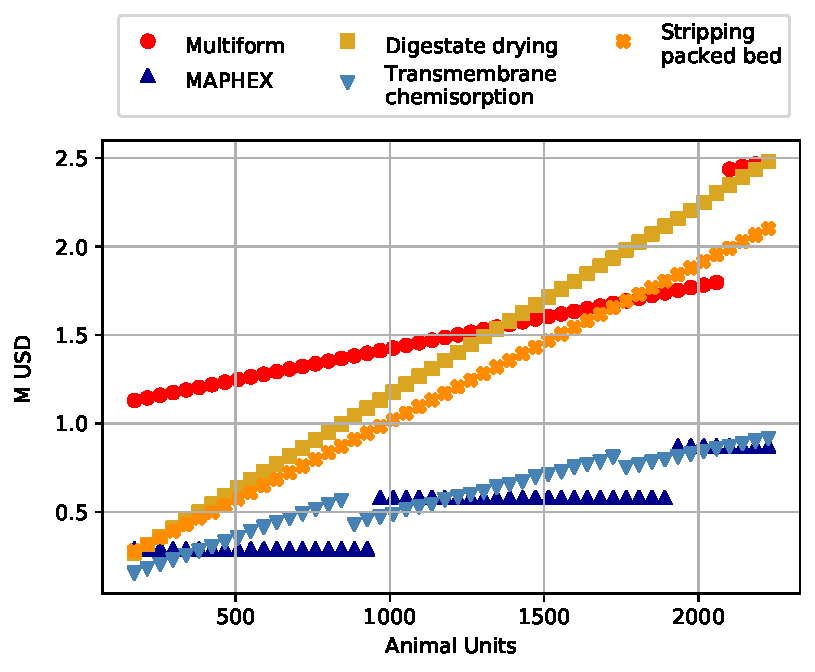
\includegraphics[width=1\linewidth, trim={0cm 0cm 0cm 0cm},clip]{gfx/AppendixD/EquipCost.pdf} 
		\caption{CAPEX}
		\label{fig:CAPEX}
	\end{subfigure}

	\bigskip

	\begin{subfigure}[t]{0.7\textwidth}
		\centering
		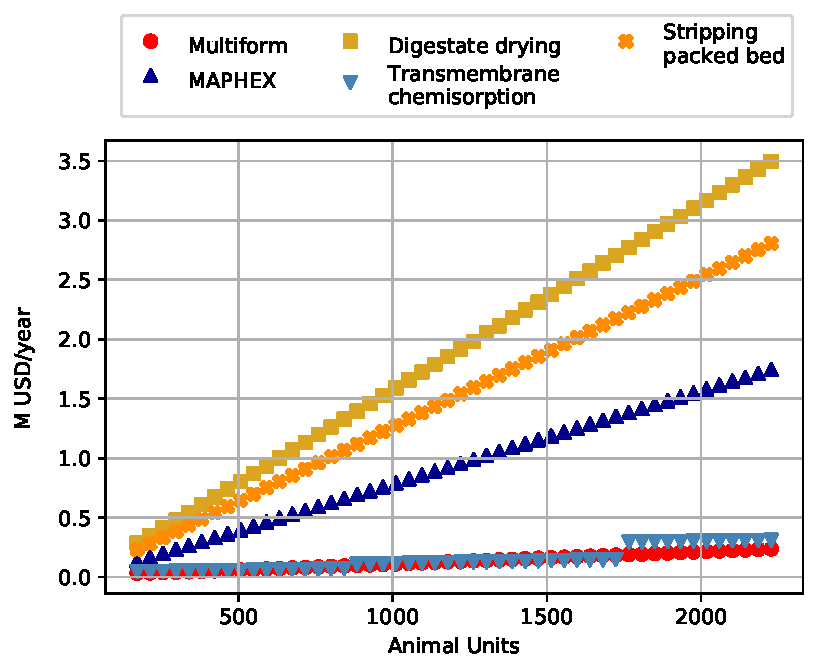
\includegraphics[width=1\linewidth, trim={0cm 0cm 0cm 0cm},clip]{gfx/AppendixD/OpCost.pdf} 
		\caption{OPEX}
		\label{fig:OPEX}
	\end{subfigure}
	
	\caption{CAPEX and OPEX of the assesed nitrogen recovery technologies, including the cost of anaerobic digestion stage.} \label{fig:CAPEXOPEX}
\end{figure}

\newpage

\begin{figure}[h!]
	\centering 
	\begin{subfigure}[t]{0.7\textwidth}
		\centering
		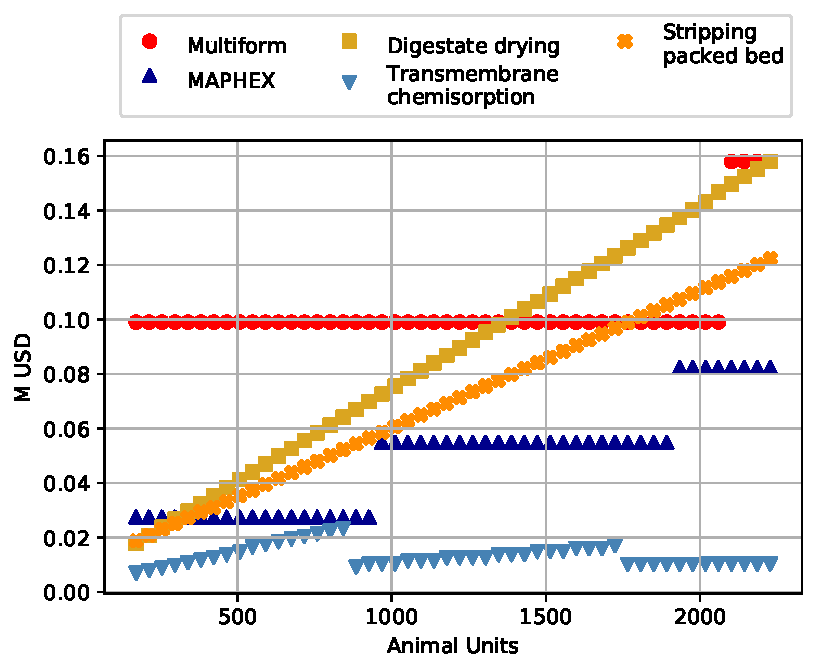
\includegraphics[width=1\linewidth, trim={0cm 0cm 0cm 0cm},clip]{gfx/AppendixD/EquipCost_NoAD.pdf} 
		\caption{CAPEX}
		\label{fig:CAPEX_NoAD}
	\end{subfigure}

	\bigskip

	\begin{subfigure}[t]{0.7\textwidth}
		\centering
		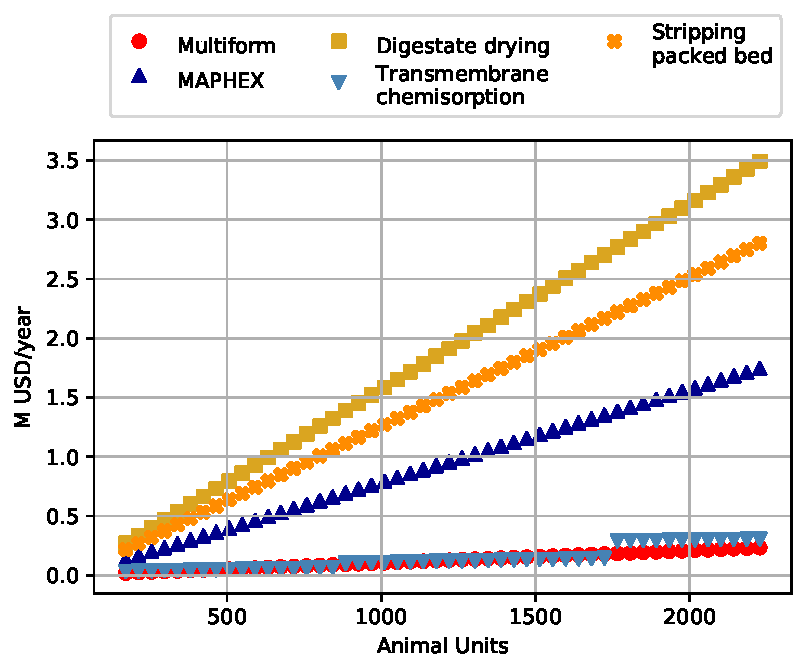
\includegraphics[width=1\linewidth, trim={0cm 0cm 0cm 0cm},clip]{gfx/AppendixD/OpCost_NoAD.pdf} 
		\caption{OPEX}
		\label{fig:OPEX_NoAD}
	\end{subfigure}
	
	\caption{CAPEX and OPEX of the assesed nitrogen recovery technologies, excluding the cost of anaerobic digestion stage.} \label{fig:CAPEXOPEX_NoAD}
\end{figure}

\newpage

\section{Processing cost}
\begin{figure}[h!]
	\centering 
	\begin{subfigure}[t]{0.7\textwidth}
		\centering
		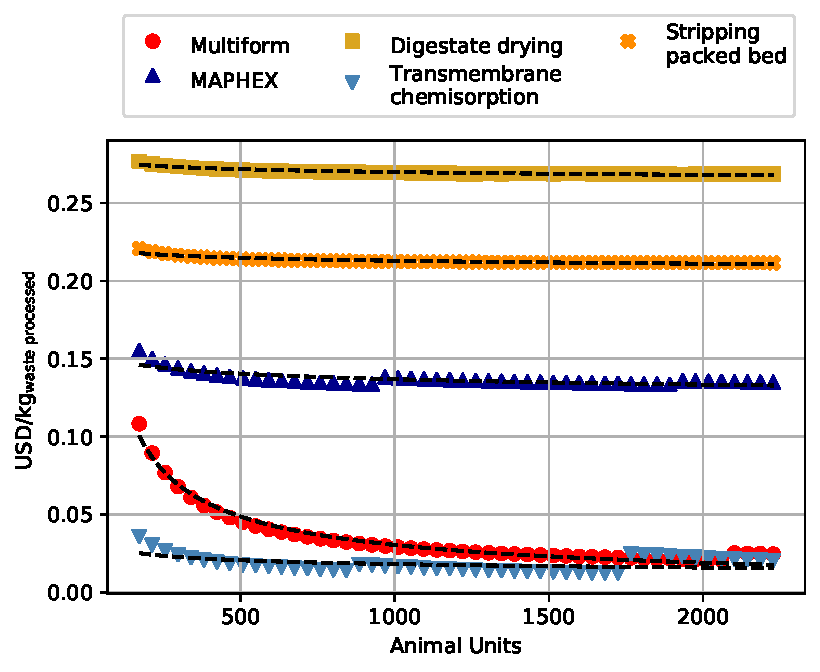
\includegraphics[width=1\linewidth, trim={0cm 0cm 0cm 0cm},clip]{gfx/AppendixD/ScaleUp2WasteProcCost_NoAD.pdf} 
		\caption{Waste processing cost}
		\label{fig:ScaleUp2WasteProcCost_NoAD}
	\end{subfigure}

	\bigskip

	\begin{subfigure}[t]{0.7\textwidth}
		\centering
		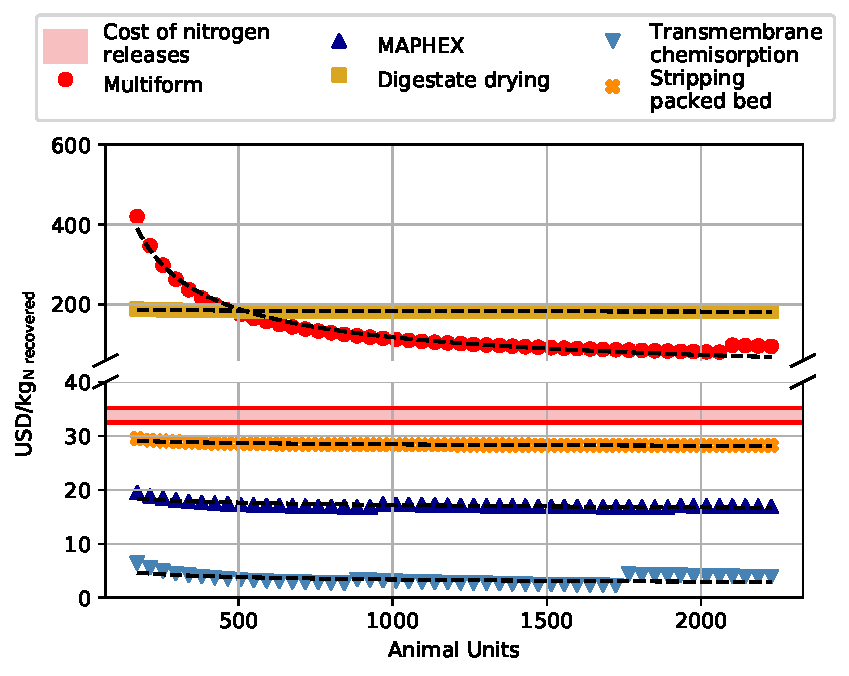
\includegraphics[width=1\linewidth, trim={0cm 0cm 0cm 0cm},clip]{gfx/AppendixD/ScaleUp2_NoAD.pdf} 
		\caption{Nitrogen recovery cost}
		\label{fig:ScaleUp2_NoAD}
	\end{subfigure}
	
	\caption{Processing cost for different livestock facility sizes, excluding the cost of anaerobic digestion stage.} \label{fig:ScaleUGlobal_NoAD}
\end{figure}

\newpage

\begin{table}[h!] 
	\centering
	\caption{Correlations to estimate the processing cost of the evaluated technologies as a function of animal units ($AU$), excluding the cost of anaerobic digestion stage.} \label{table:ScaleUpCorrelations_NoAD}
	\resizebox{\columnwidth}{!}{
	\begin{tabular}{@{}cccc@{}}
		\toprule
		\multirow{2}{*}{System} & &\multicolumn{1}{c}{\begin{tabular}[c]{@{}c@{}}Waste processing cost\\  $\left(\sfrac{\text{USD}}{\text{kg}_{\text{waste processed}}}\right)$\end{tabular}} & \multicolumn{1}{c}{\begin{tabular}[c]{@{}c@{}}Total nitrogen recovery cost\\  $\left(\sfrac{\text{USD}}{\text{kg}_{\text{N recovered}}}\right)$\end{tabular}} \\ \cmidrule(l){3-3}\cmidrule(l){4-4} 
		& Correlation                           & Parameters                &                           Parameters                      \\  \midrule
		%		\cmidrule(l){2-3}
		%		\cmidrule(r){1-1}
		Digestate drying  
		& \multirow{13}{*}{$C = a \cdot AU^{b}$}               
		& \begin{tabular}[c]{@{}c@{}}$a$=0.289\\ $b$=-0.00974\end{tabular}  
		& \begin{tabular}[c]{@{}c@{}}$a$=196.534\\ $b$=-0.00974\end{tabular}            \\\\
		Multiform         
		&                                       
		& \begin{tabular}[c]{@{}c@{}}$a$=3.261\\ $b$=-0.676\end{tabular}         
		& \begin{tabular}[c]{@{}c@{}}$a$=12660.077\\ $b$=-0.676\end{tabular}       \\\\
		MAPHEX            
		&                                       
		& \begin{tabular}[c]{@{}c@{}}$a$=0.177 \\ $b$=-0.0372   \end{tabular}       
		& \begin{tabular}[c]{@{}c@{}}$a$=22.240 \\ $b$=-0.0372   \end{tabular}                                             \\ \\ 
		\begin{tabular}[c]{@{}c@{}}Stripping in \\ packed tower  \end{tabular}             &                                       
		& \begin{tabular}[c]{@{}c@{}}$a$=0.233 \\ $b$=-0.0128  \end{tabular}        & \begin{tabular}[c]{@{}c@{}}$a$=31.089 \\ $b$=-0.0128  \end{tabular} \\ \\ 
		Membrane            
		&                                       
		& \begin{tabular}[c]{@{}c@{}}$a$=0.0410 \\ $b$=-0.135  \end{tabular}        
		& \begin{tabular}[c]{@{}c@{}}$a$=7.488 \\ $b$=-0.132  \end{tabular}  \\
		\bottomrule 
	\end{tabular}
}
\end{table}

\newpage

\section*{Bibliography}
\addcontentsline{toc}{section}{Bibliography}

\printbibliography[heading=none]
\end{refsection}
%\begin{lstlisting}[float=b,language=Pascal,frame=tb,caption={A floating example (\texttt{listings} manual)},label=lst:useless]
%for i:=maxint downto 0 do
%begin
%{ do nothing }
%end;
%\end{lstlisting}

